\en

\section{Code Duplication Detection}

Code Duplication Detection is a field in computer science that has attracted
researchers' attention since 1988~\citep{firstman}. Code
duplication is considered a harmful artifact in software, as it negatively
affects tasks such as code readability and increases the likelihood of
introducing bugs~\citep{harmone}. In most cases, code duplication tends to make
software more unstable than its non-duplicated counterpart~\citep{harmtwo}.

Over the years, research on Code Duplication Detection has branched into two
main areas: Code Clone Detection and Code Plagiarism Detection. The former
focuses on technical aspects, while the latter incorporates social dimensions
into the research field~\citep{litreview}. In this work, we focus solely on the
Code Clone Detection branch due to the nature of our study.


\subsection{Diff command}

The \textit{diff} command is a command line in GNU/Linux that allows the user to compare 
two files line by line~\citep{diffcommand}. There are multiple forms in which the command 
results can be shown to the user, and Figure \ref{fig:diff} shows one of them. 
With the command results, it is easy to visualize and extract the number of lines that 
are equal and different between the two compared files.

\begin{figure}
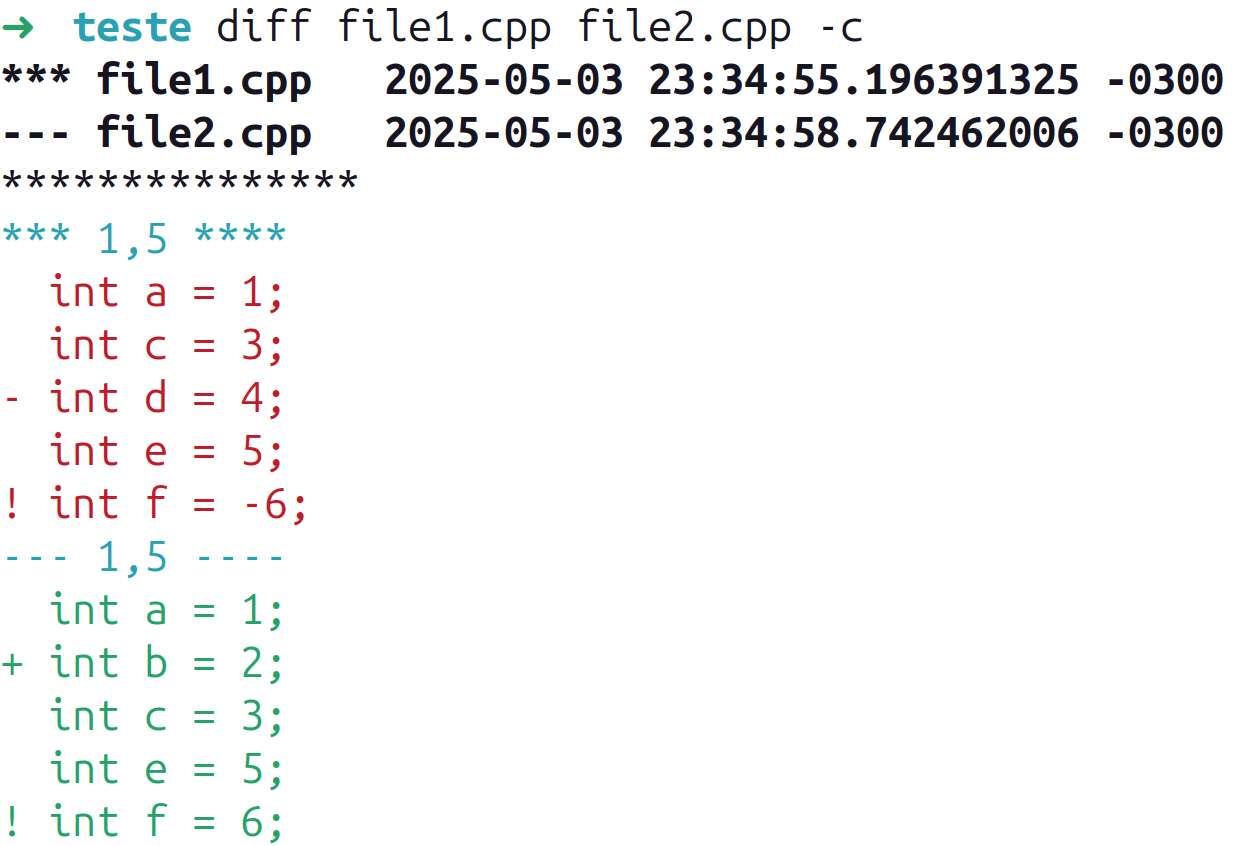
\includegraphics[scale=0.2]{diff_command}
\caption[Example of \textit{diff} command executed]{
Example of \textit{diff} command executed
\footnote{
File 1 content is shown in red, and File 2 content is shown in green. \textit{-} 
represents a line that only exists in file 1, \textit{+} represents a line that only 
exists in file 2,\textit{!} represents a line that exists in both files but has modifications 
between them, and empty at the start of a line represents that the line exists in 
both files without any modifications.
}
}
\label{fig:diff}
\end{figure}

We use the \textit{diff} command as the base of one of the code duplication detection 
methods on the tool proposed in this work, although it is not explored as the text 
similarity method chosen for code duplication detection.

\subsection{Types of Code Clone Duplication}
\label{subsec:types}

Classifying two code artifacts as duplicates raises the question of
what constitutes duplication. To address this, the literature categorizes code
duplication based on the extent of differences between code artifacts,
resulting in four types of code clone duplications~\citep{litreview}. When
comparing two code artifacts, F and G, the four types of code duplication can
be described as follows~\citep{litreview}:

\begin{itemize}
    \begin{item}
	\textbf{Type-1 (T1):} The differences between F and G are limited to
	    changes in comments, variable names, white spaces, and other
	    irrelevant elements. Figure~\ref{fig:type1} shows a typical example
	    of Type-1 clone duplication~\citep{litreview}.
    \end{item}
    \begin{item}
	\textbf{Type-2 (T2):} The differences between F and G include those
	    from Type-1, along with the addition and deletion of redundant
	    code. Figure~\ref{fig:type2} shows a typical example of Type-2 code
	    clone duplication~\citep{litreview}.
    \end{item}
    \begin{item}
	\textbf{Type-3 (T3):} The differences between F and G include those
	    from Type-2, as well as reordering code blocks and statements
	    within code blocks. Figure~\ref{fig:type3} shows a typical example
	    of Type-3 code clone duplication~\citep{litreview}.
    \end{item}
    \begin{item}
	\textbf{Type-4 (T4):} The differences between F and G include those
	    from Type-3, along with changes in data structures, the order of
	    operands/operators in expressions, or the replacement of code parts
	    with equivalent compositions. Figure~\ref{fig:type4} shows a
	    typical example of Type-4 code clone duplication~\citep{litreview}.
    \end{item}
\end{itemize}

\begin{figure}[ht]
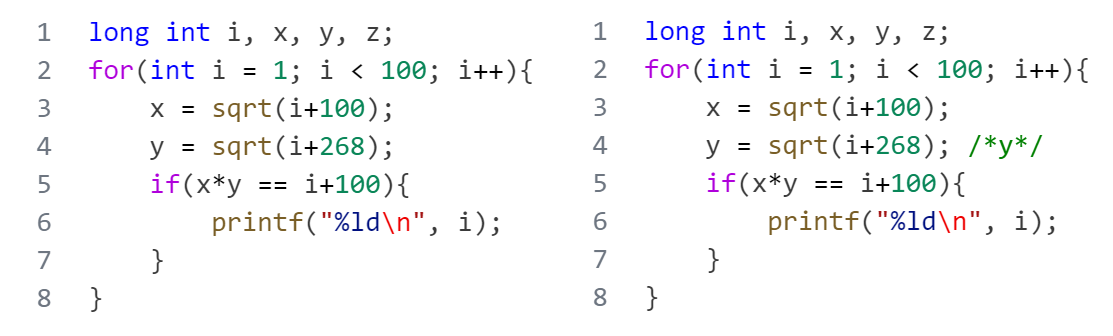
\includegraphics[scale=0.38]{types/type1}
\caption{Example of Type-1 code clone duplication~\citep{litreview}.}
\label{fig:type1}
\end{figure}

\begin{figure}[ht]
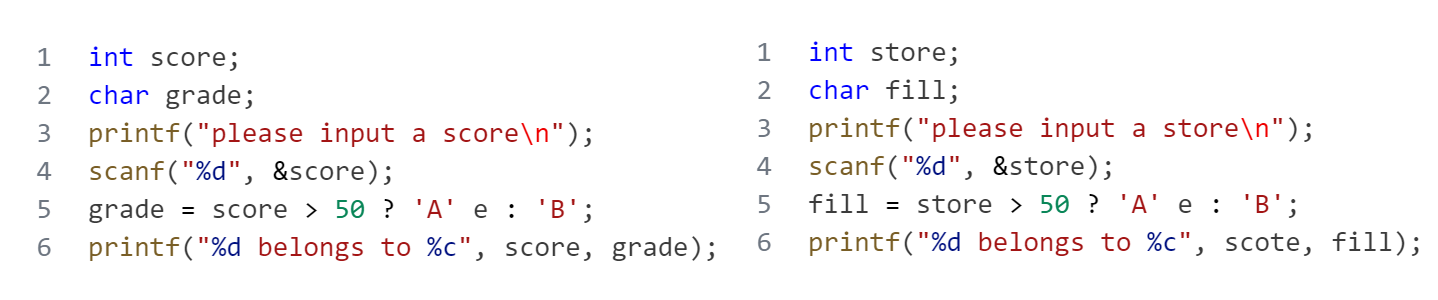
\includegraphics[scale=0.38]{types/type2}
\caption{Example of Type-2 code clone duplication~\citep{litreview}.}
\label{fig:type2}
\end{figure}

\begin{figure}[ht]
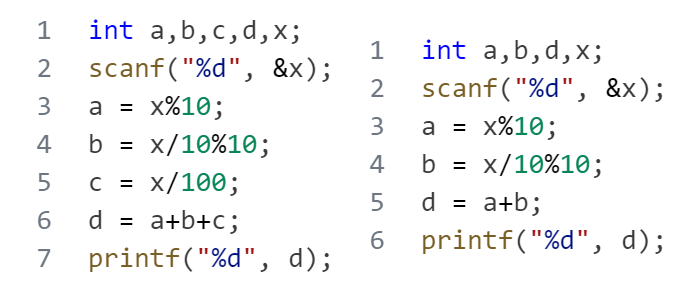
\includegraphics[scale=0.38]{types/type3}
\caption{Example of Type-3 code clone duplication~\citep{litreview}.}
\label{fig:type3}
\end{figure}

\begin{figure}[ht]
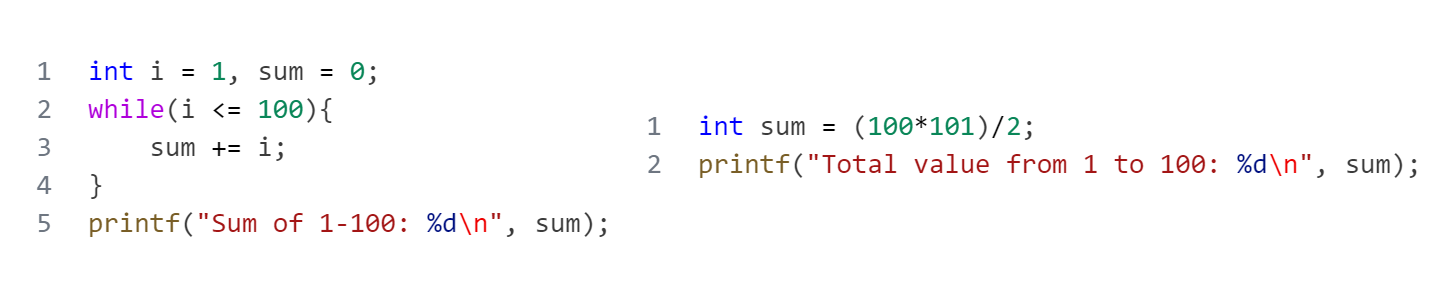
\includegraphics[scale=0.38]{types/type4}
\caption{Example of Type-4 code clone duplication~\citep{litreview}.}
\label{fig:type4}
\end{figure}


\subsection{Literature Approaches for Code Clone Detection}

Over time, various techniques and methods have been developed in the literature
to address the code clone detection problem. For better analysis and
understanding, these approaches are categorized into five methodologies based
on their characteristics \citep{litreview}:

\begin{itemize}
    \item \textbf{Textual-based approaches:} According to Chen’s literature 
    review \citep{litreview}, this is the earliest methodology explored in 
    the field. It treats code as a text artifact and applies textual similarity
    techniques. An example is the work of~\cite{textexample}, 
    which uses parsing and grammar techniques to detect code clones.

    \item \textbf{Token-based approaches:} This method tackles the problem 
    similarly to lexical analysis in the compilation process \citep{litreview}. 
    It involves identifying programming language tokens such as constants and 
    keywords, mapping variables to independent representations, etc. An example
    is the work of~\cite{tokenexample}, which detects code 
    clones through hashed token sequences.

    \item \textbf{Tree-based approaches:} While token-based approaches utilize
     lexical analysis, tree-based approaches rely on syntax trees, which store
     semantic information of code artifacts based on the programming
     language~\citep{compiler}. An example of this approach is the work of~\cite{treeexample}.

    \item \textbf{Metric-based approaches:} This methodology uses extracted 
    metrics from code artifacts as embedding representations to measure 
    similarity~\citep{litreview}, akin to the Word2Vec model by~\cite{wordtovec}.
    Metrics can include program size, number of variables, 
    memory access counts, etc. An example is the work of~\cite{metricexample}.

    \item \textbf{Graph-based approaches:} Similar to tree-based approaches, 
    this methodology depends on intermediate program representations, 
    specifically the program dependence graph (PDG), which stores information 
    on control, statements, and data dependencies~\citep{prodg}. A recent 
    example is the work of~\cite{tailor}, which represents one of 
    the state-of-the-art works in the field.
\end{itemize}

State-of-the-art code clone detection methods typically require substantial
computational time and memory, and many are language-specific, limiting their
applicability across different programming languages~\citep{litreview}. Given
these constraints, we opted for a generalist textual-based approach using
Natural Language Processing (NLP) text similarity methods, which we will
introduce in Chapter~\ref{cha:tool} and evaluate in this work.

\subsection{Evaluating Code Duplication Methods}

\label{subsec:codemethods}

To evaluate and compare code clone detection methods, two widely adopted
datasets are available: OJ-Clone, collected from a pedagogical online judge
system~\citep{ojclone}, and BigCloneBench, compiled from over 25,000 Java
software systems~\citep{bigclonebench}. However, literature has expressed
concerns over the limited scope of OJ-Clone and the issues with BigCloneBench
identified by~\cite{bigfail}. Despite these
limitations, BigCloneBench is commonly used due to the limited pedagogical
scope of OJ-Clone.

BigCloneBench further divides Type-3 duplications into three categories: Weak
Type-3 (WT3), Medium Type-3 (MT3), and Strong Type-3 (ST3); where WT3 is closer
to Type-4 and ST3 is closer to Type-2~\citep{bigclonebench}. This results in
six possible outcomes for a code pair: Type-1, Type-2, Strong Type-3, Medium
Type-3, Weak Type-3/Type-4, and non-duplicate~\citep{bigclonebench}.

To assess code clone detection methods against these datasets, researchers
calculate metrics based on the model’s predictions. There are four possible
outcomes for each prediction:

\begin{itemize}
    \begin{item}
        \textit{True Positivity (TP):} The model correctly identifies an instance as a code clone.
    \end{item}
    \begin{item}
        \textit{False Positivity (FP):} The model incorrectly identifies a non-clone instance as a code clone.
    \end{item}
    \begin{item}
        \textit{True Negative (TN):} The model correctly identifies an instance as non-clone.
    \end{item}
    \begin{item}
        \textit{False Negative (FN):} The model incorrectly identifies a clone instance as non-clone.
    \end{item}
\end{itemize}

Using the counts of TP, FP, TN, and FN, standard metrics such as Precision,
Recall, and F-Score can be calculated~\citep{recall}. In this work, we focus on
the Recall metric, which is commonly reported in literature for comparing code
clone detection approaches. Recall is defined as follows~\citep{recall}:

$$Recall = \frac{\sum TP}{\sum TP + \sum FN }$$

Where $\sum TP$ is the total number of true positives, and $\sum FN$ is the
total number of false negatives. Recall values range between 0 and 1, with
values closer to 1 indicating better performance.

